\documentclass[12pt]{article}

% set margins and spacing
\addtolength{\textwidth}{1.3in}
\addtolength{\oddsidemargin}{-.65in} %left margin
\addtolength{\evensidemargin}{-.65in}
\setlength{\textheight}{9in}
\setlength{\topmargin}{-.5in}
\setlength{\headheight}{0.0in}
\setlength{\footskip}{.375in}
\renewcommand{\baselinestretch}{1.0}
\linespread{1.0}

% load miscellaneous packages
\usepackage{csquotes}
\usepackage[american]{babel}
\usepackage[usenames,dvipsnames]{color}
\usepackage{graphicx,amsbsy,amssymb, amsmath, amsthm, MnSymbol,bbding,times, verbatim,bm,pifont,pdfsync,setspace,natbib}
\usepackage{float}

% enable hyperlinks and table of contents
\usepackage[pdftex,
bookmarks=true,
bookmarksnumbered=false,
pdfview=fitH,
bookmarksopen=true,hyperfootnotes=false]{hyperref}

% define environments
\newtheorem{definition}{Definition}
\newtheorem{fact}{Fact}
\newtheorem{result}{Result}
\newtheorem{proposition}{Proposition}



\begin{document}
\title{Shifting Revenue Strategy: The Inverse Relationship Between Consumption Tax and Tariff Revenue in Developed and Developing Countries}
\author{Kathryn Sarrge\thanks{Syracuse University, Economics Students. Email: kesarrge@syr.edu} \and Dylan Thomas\thanks{dthoma26@syr.edu} \and Umar Bilgrammi\thanks{ujbilgra@syr.edu}}
\date{\vskip-.1in \today}
\maketitle

\vskip.3in
\begin{center} {\bf Abstract} \end{center}

\begin{quote}
{\small We investigate the relationship between consumption taxes such as Value Added Tax (VAT) and tariffs in developing and developed countries, with the aim of understanding the fiscal strategies employed by both developing and developed countries. Specifically, we explore whether there exists an inverse relationship between consumption tax and tariff revenue, hypothesizing that as consumption taxes like VAT increases, tariff revenue decreases. Utilizing data from the World Integrated Trade Solution (WITS) database, covering 194 countries from 1988 to 2022, we analyze the two forms of taxation as a percentage of government revenue and consider their implications for economic development. Our findings reveal a moderate negative correlation between VAT and tariff revenue in developing and developed countries, with a correlation coefficient of -0.3255, indicating that as countries shift towards consumption-based taxes like VAT, their reliance on tariffs decreases. Our research discusses these findings within the context of broader tax reform literature, analyzing the relationship of shifting from trade taxes to consumption taxes.}
\end{quote}

\bigskip
\section{Introduction} \label{sec:introduction}
The generation of government revenue plays a vital role in shaping a country's economic stability and growth. Methods to generate revenue vary by country due to various factors including laws, border policies, and a country's economic strengths. According to Michael et al. (1993), for many countries, consumption taxes on goods and services such as Value Added Tax (VAT) and tariffs on international trade are key revenue sources. Understanding the relationship between these two forms of taxation, including whether they are complements or substitutes, can offer valuable insights for policymakers looking to optimize tax policies in search of overall national development. Our findings suggest that there is a negative correlation between consumption taxes like VAT and tariffs in both developing and developed countries. 

This topic is especially important because the reliance on tariffs has historically been higher in developing countries, but as these countries modernize and integrate into the global economy, we may observe a shift towards other forms of taxation, such as VAT. By analyzing this relationship, we aim to provide critical insights into how governments balance their revenue sources.

This study investigates the relationship between taxes on goods and services and taxes on international trade in developed and developing countries. The primary research question is: Is there an inverse relationship between VAT revenue and tariff revenue in developed and developing countries? Specifically, we hypothesize  if consumption tax such as VAT increases in a developed or developing country, then tariffs decrease. We will examine data from the World Integrated Trade Solution (WITS) database, which provides information on both forms of taxation as a percentage of government revenue across 194 countries from 1988 to 2022. By analyzing these two key revenue sources, we hope to better understand the fiscal strategies employed by developing and developed nations.

In this paper, we will present a detailed analysis of the data collected from the WITS database, which includes not only taxes on goods and services and tariffs but also GDP per capita to help classify countries as developed or developing. We will start with a description of the data and its sources, followed by a theoretical discussion of the relationship between VAT and tariffs. The results section will outline the correlation between these variables and provide a series of visualizations to illustrate the relationships found in the data. Finally, the paper will conclude with a discussion of the findings, their implications for developing and developed country's fiscal policy, and areas for further research.

\section{Literature Review} \label{sec:literature}

The literature on the relationship between tariffs, and consumption taxes offers a range of insights, particularly in the context of developing countries. Many studies suggest that reducing tariffs while increasing consumption taxes, such as Value Added Tax (VAT), can improve welfare and maintain or even enhance government revenue. However, challenges such as the informal economy and political resistance complicate these reforms.

Michael et al. (1993) explore the potential benefits of tax reforms in developing countries, emphasizing the shift from inefficient tariffs to more efficient consumption taxes like VAT. They conclude that such reforms can indeed improve welfare, supporting our hypothesis that reducing tariffs while increasing VAT can stabilize government revenue and improve welfare. Similarly, Waglé (2011) models the shift from trade taxes to domestic consumption taxes, finding that this transition is not only feasible but also beneficial for revenue stability, provided that enforcement mechanisms are in place. These findings align with our study’s focus on the relationship between VAT and tariffs.

John Mark Hansen (1990) takes a political economy perspective, explaining how tariffs have historically been used by governments, especially in developing countries, as tools for economic advantage. However, he argues that as countries modernize, reliance on tariffs becomes increasingly inefficient. This insight is important for understanding the political challenges that may hinder the reduction of tariffs in favor of consumption taxes, a point that complicates our analysis of the benefits of tax reforms.

Thuy Tien Ho, Xuan Hang Tran, and Quang Khai Nguyen (2023) investigate the link between tax revenue, economic growth, and trade openness, with a focus on developing countries. While they do not explicitly explore the relationship between VAT and tariffs, their findings on the importance of trade openness for economic growth help contextualize our study. Increased trade openness, facilitated by tariff reductions, can potentially support the shift to VAT as a more stable source of revenue, reinforcing the idea that reducing tariffs can have broader positive effects on economic performance.

Emran and Stiglitz (2005) provide a cautionary perspective, highlighting the challenges of implementing VAT reforms in developing countries due to the informal economy. Their research suggests that while the shift from tariffs to VAT could theoretically enhance revenue, the effectiveness of VAT is often undermined by underreporting and evasion. This insight introduces a critical consideration for our research, as it suggests that simply increasing VAT may not lead to the desired outcomes without addressing informal economic activities. Additionally, Kowalski's (2005) paper examines how changes in tariff rates impact government revenue in developing countries, highlighting the critical role that tariff reforms play in shaping fiscal policy. The study is important for understanding the potential consequences of reducing tariff reliance and supports the argument that developing countries need to find alternative revenue sources, such as VAT, to maintain stable government finances.

The general consensus in the literature is that reducing tariffs and increasing consumption taxes can enhance revenue and welfare, but the success of these reforms depends on a variety of factors. Studies like those of Michael et al. (1993) and Waglé (2011) support the view that such reforms can be beneficial, while Hansen’s (1990) political economy perspective highlights the difficulties of overcoming entrenched tariff policies. Emran and Stiglitz’s (2005) concerns about the informal economy introduce another layer of complexity, suggesting that reforms must be carefully designed and implemented. Ho et al. (2023) provide a broader context by emphasizing the role of trade openness in fostering economic growth, aligning with our study’s focus on the impact of tariff reductions.

In summary, the literature provides a nuanced view of the relationship between VAT, tariffs, and economic welfare. While most studies support the idea that reducing tariffs and increasing VAT can improve revenue and welfare, they also highlight the importance of political will, effective enforcement, and addressing the informal economy. Our research builds on these findings by specifically examining the inverse relationship between VAT and tariff revenue, contributing to the ongoing discussion of tax reforms in developing countries.

\section{Theoretical Analysis}
\label{sec:theory}
The relationship between consumption taxes like VAT and tariffs is central to understanding how developing countries structure their tax systems. Generally, VAT is considered a more stable and efficient source of revenue than tariffs, especially as countries modernize their taxation (Kowalski, P. 2005). Tariffs, which are taxes imposed on imports, are often seen as a tool for protecting domestic industries but can be disruptive to trade and economic efficiency. In contrast, consumption taxes are levied on consumption and can be easier to collect, particularly when countries have established taxation systems. As countries develop, it is expected that they may shift from relying on tariffs to more consumption-based taxes like VAT.

We hypothesize that there is a negative correlation between consumption taxes like VAT and tariff revenue in either developed or developing countries. Specifically, we expect that as VAT revenue increases (indicating a shift towards a modern tax system), tariff revenue will decrease. Therefore, our null hypothesis is that increases in consumption taxes like VAT have no effect on tariffs in developed or developing countries. 
The shift between consumption taxes like VAT increasing as a percent of revenue while tariffs decrease as a percent of revenue could reflect a broader trend of economic liberalization and integration into global trade, where countries increasingly adopt consumption taxes as part of their fiscal strategies and reduce their reliance on trade taxes. We also anticipate that the relationship between consumption taxes and tariffs may vary depending on a country's level of economic development, which we control for using GDP per capita.

This hypothesis is grounded in the theory of tax modernization, where governments gradually move away from potentially risky taxes like tariffs and towards more efficient and broad-based taxes consumption taxes like VAT (Kowalski, P. 2005). By examining this relationship, we aim to better understand the fiscal landscape of developing and developed countries.

\section{Data}
\label{sec:data}

We analyzed three time series data sources from the \href{https://wits.worldbank.org/CountryProfile/en/Country/BY-COUNTRY/StartYear/1988/EndYear/2022/Indicator/GC-TAX-GSRV-VA-ZS}{World Integrated Trade Solution} website, which provides detailed information about taxes and tariffs as a percentage of revenue for developing and developed countries, while using a third variable, GDP per capita. These variables span from 1988 to 2022 and cover 194 countries. The variables we focus on represent two distinct types of revenue sources for these countries: taxes on goods and services and taxes on international trade. The third dataset is simply used for identifying countries as developed or developing based on their GDP per capita in current US dollars. 

The WITS database aggregates data from various sources. It primarily compiles national statistics on tariffs and taxes from government reports and international organizations. The data collection process involves gathering information directly from the national governments' reports, which are often based on their domestic economic activities, tax laws, and trade statistics. Additionally, the data may be supplemented by international organizations like the International Monetary Fund (IMF), World Bank, and the United Nations, who collect national statistics to ensure comparability across countries.

The collection of this data is subject to the availability and reliability of national statistical offices, and differences may arise depending on the country’s data reporting practices. While the dataset provides information for most countries, certain nations may have incomplete or missing data for specific years. In these cases, either the data is unavailable for that particular year or there are gaps due to inconsistencies in national reporting. For some countries, the data may not start until a later year, and for others, the data may be missing intermittently across the 34-year period.

In this study, we focus on developing countries, where taxes and tariffs play a crucial role in government revenue. However, there is variation in how governments rely on different revenue sources. We acknowledge that the dataset is limited to the data available from the WITS platform, and some countries may have more reliable, consistent reporting than others. For example, developed countries often have more accurate and complete records, while developing countries may face challenges in data collection or reporting.

The variables we use in our data are taxes on goods and services, taxes on international trade, and GDP per capita. Taxes on goods and services as a percent of revenue represent the percentage of revenue from taxes like VAT or sales taxes as a percentage of total revenue. It includes taxes levied on consumption, which can vary greatly across countries, especially in the form of Value Added Taxes (VAT) or other consumption-based taxes. Taxes on international trade as a percentage of revenue represent the revenue from tariffs as a percentage of total revenue, reflecting the importance of international trade in a country's economic structure. Finally, GDP per capita represents a country's gross domestic product divided by its population, which can be considered a decent indicator of the standard of living in a country. In our project specifically, GDP per capita will be used to identify developing and developed countries. Country's that are developed will have a GDP per capita of greater than 12,000 current USD. Countries that are developing with have a GDP per capita that is less than or equal to 12,000 current USD (Freed, Jeffrey S, et al, 2020). For the purpose of our research, countries are evaluated on a year by year basis, therefore a country may be considered developing or developed depending on the year. 

The summary statistics for the three variables- taxes on goods and services, taxes on international trade, and gross domestic product—are presented in the table below. This table provides an overview of the mean, standard deviation, minimum, and maximum values for these variables across all countries and years in the dataset.



These statistics reflect the general range of taxes and tariffs as a percentage of government revenue. It is important to note that these figures represent averages across developing and developed countries, with significant variation between individual countries.

\section{Results}
\label{sec:result}

In this section, we present the analysis of the relationship between taxes on consumption like Value Added Tax (VAT) and taxes on international trade (tariffs) in developing countries, as described in Section 4. Our primary focus is to investigate the potential inverse relationship between VAT revenue and tariff revenue, and to understand the trends over time. We will first look at descriptive statistics, followed by graphical evidence, and then analyze time-series trends and correlations. 

Table 1 provides summary statistics for our three key variables: international tax, consumption tax, and Gross Domestic Product (GDP). Both international tax and consumption tax are expressed as percentages of total revenue, while GDP is measured in current U.S. dollars. The mean for both international tax and consumption tax is strikingly similar, at approximately 10.24 percent and 10.26 percent, respectively. However, there are notable differences in their distributions.

{
\def\sym#1{\ifmmode^{#1}\else\(^{#1}\)\fi}
\begin{tabular}{l*{1}{ccccc}}
            &\multicolumn{5}{c}{}                                         \\
            &\multicolumn{5}{c}{}                                            \\
            &       count&        mean&          sd&         min&         max\\
\hline
international&        2969&    10.24049&    11.61363&   -.1304207&    64.65984\\
gdp         &        6499&    11320.32&     17465.2&    22.85037&    133590.1\\
consumption &        3211&    10.25779&    5.280867&    .0329885&    40.00499\\
\hline
\end{tabular}
}

Table 1 provides summary statistics for our three variables: international tax, consumption tax, and gross domestic product, with international and consumption tax in terms of percent of revenue and gross domestic production in terms of current U.S. dollars. The means for both international tax and consumption tax are extremely similar while the standard deviation for international tax is nearly double of consumption tax, meaning there are substantial differences in how these variables differ from their means.

International tax has a maximum of 64.66 percent, while consumption tax only has a maximum of 40.00 percent, indicating that international taxes can make up a larger portion of revenue in some countries, especially those with extreme tariff rates. Additionally, international tax has a higher standard deviation (11.61 percent) compared to consumption tax (5.28 percent), which suggests that international tax revenue is more volatile across countries.

The pairwise correlation coefficient test between the international tax and the consumption tax is -.3255. Therefore, these variables have a moderate strength negative correlation. This shows that there is a statistically significant negative relationship between tariffs and consumption taxes in developing and developed countries. Thus, we reject the null hypothesis that there is no relationship between these two variables. 

A graphical visualization of the whole data is best represented by Figure 1; a scatterplot including international and consumption data. A line of best fit is displayed on the graph, visualizing the negative correlation between international and consumption tax. The data includes information from 194 countries from 1988 to 2022. The x-axis represents consumption tax and y-axis represents international tax, both in terms of percent of revenue. The line of best fit with a negative slope and negative correlation test indicate a moderate inverse relationship between these variables. 

\begin{figure}[h]
    \centering
    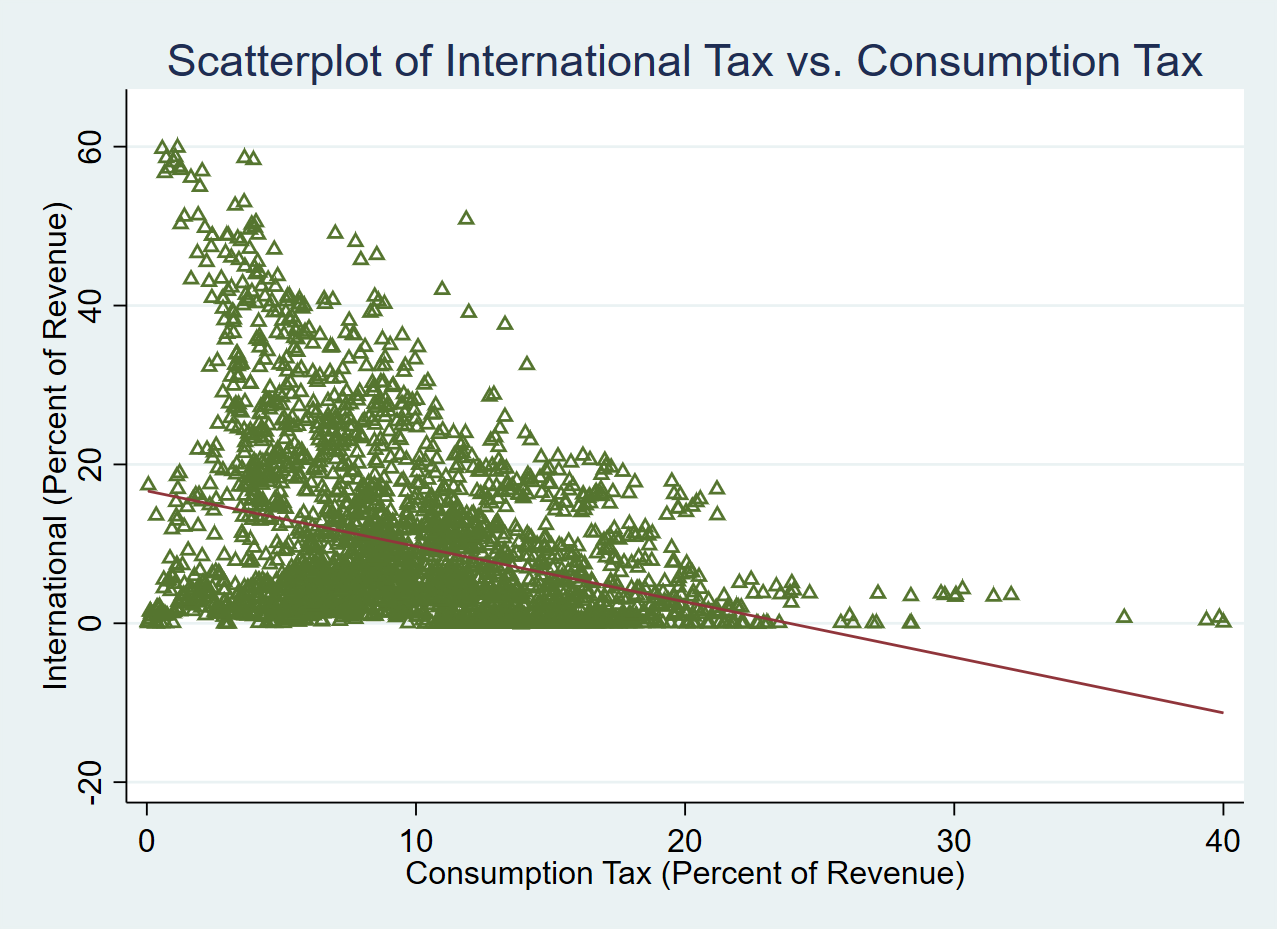
\includegraphics[width=0.5\linewidth]{Reproducibility_Package//png_files/Scatterplotintvscons.png}
    \caption{Scatterplot of International tax vs. Consumption Tax}
    \label{fig:enter-label}
\end{figure}

Figure 2 provides a direct visualization that compares international and consumption tax directly. Consumption tax has a higher density at a lower percent of revenue, while international tax seems to take a larger percent of the revenue than consumption tax at around 10 percent of revenue. 

\begin{figure}[h]
    \centering
    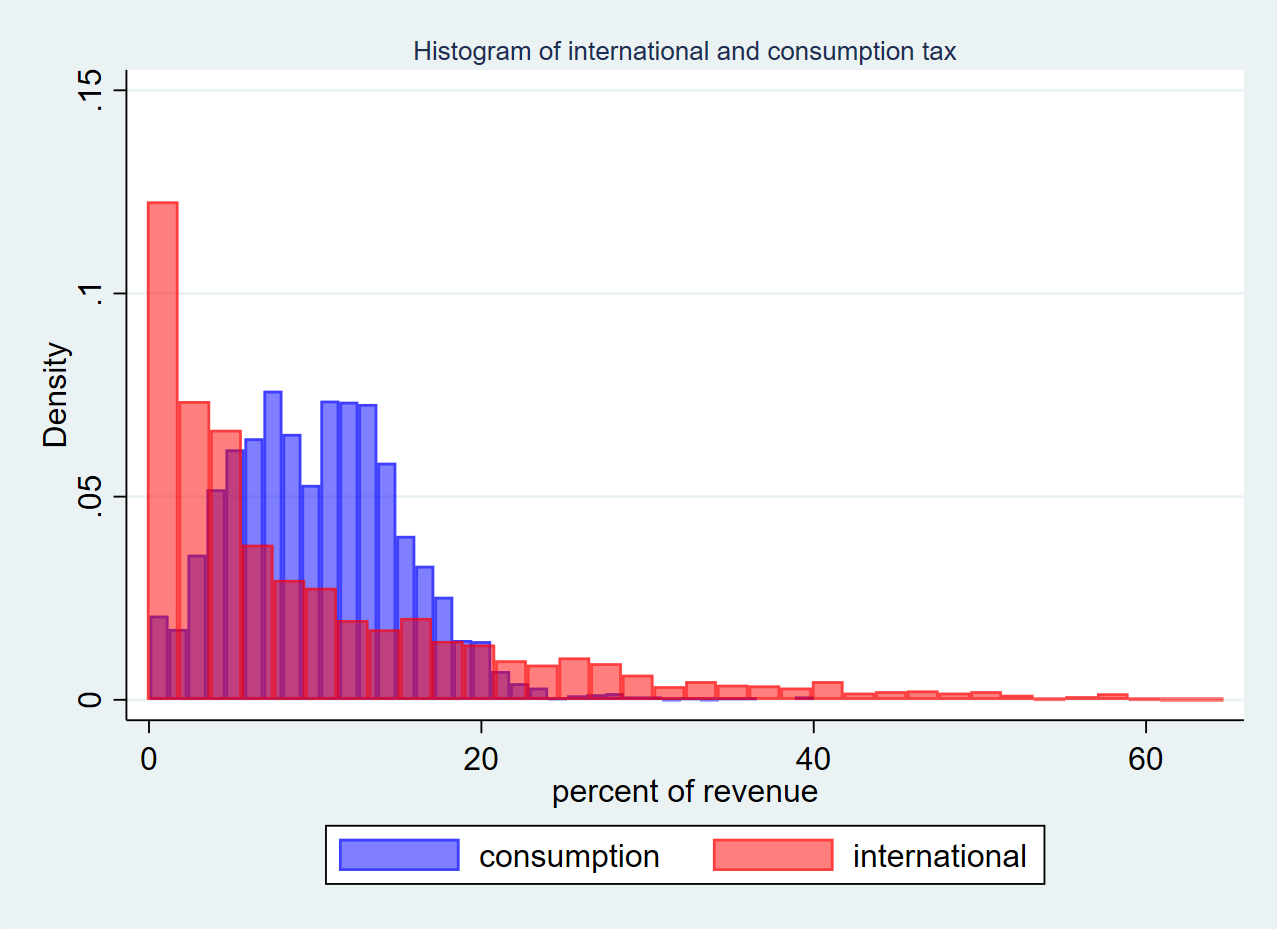
\includegraphics[width=0.5\linewidth]{Reproducibility_Package//png_files/twowayhistintcons.png}
    \caption{Histogram of International and Consumption Tax}
    \label{fig:enter-label}
\end{figure}

Figure 3 shows a histogram of international and consumption tax in only developing countries, allowing for comparisons between Figure 2 in how things differ between all countries and just developing countries. In developing countries, consumption tax and international tax seem to much more similar across more revenue percentages in comparison to Figure 2. 

\begin{figure}[h]
    \centering
    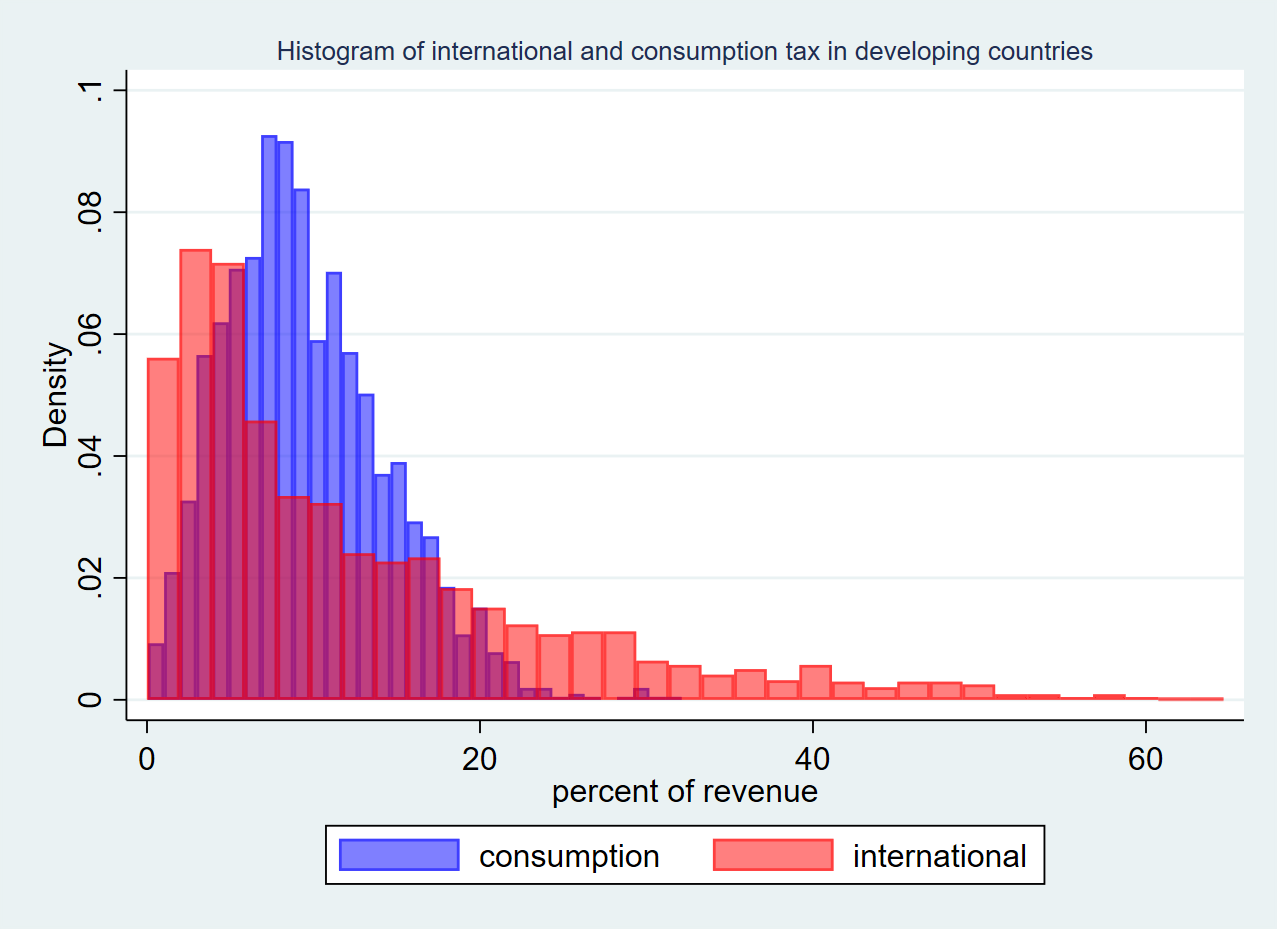
\includegraphics[width=0.5\linewidth]{Reproducibility_Package//png_files/twowayhistdevelopingintcons.png}
    \caption{Histogram of International and Consumption Tax in Developing Countries}
    \label{fig:enter-label}
\end{figure}

Figure 4 is significant as it displays the opposite trend in comparison to Figure 3. International tax has a higher density in developing countries at lower percentages of revenue in Figure 4, while Figure 3 shows that International has a lower density in developing countries at higher percentages of revenue. 

\begin{figure}[h]
    \centering
    \includegraphics[width=0.5\linewidth]{Reproducibility_Package//png_files/twowayhistdevelopedintcons.png}
    \caption{Histogram of International and Consumption Tax in Developed Countries}
    \label{fig:enter-label}
\end{figure}

While the overall trend and correlation indicate a clear relationship between consumption taxes like VAT and tariffs, there are several areas that warrant further investigation. Two particular things that we would like to look further into is specific countries and their relationship between taxes and tariffs and regional differences and how those region have different relationships with taxes and tariffs.

Country-Level Analysis: We could explore time-series graphs for individual countries, particularly those that deviate significantly from the general trend, to identify specific drivers behind these shifts. For example, countries with significant fluctuations in trade policy (e.g., trade liberalization or protectionist measures) could provide insights into how these changes affect the relationship between consumption-based taxes like VAT and tariffs.

Regional Differences: A breakdown of the data by region could shed light on whether the inverse relationship holds across different geographical areas or if regional differences play a role in the strength of this relationship.

In summary, the data suggests a moderate inverse relationship between VAT and tariff revenue in developing countries. This relationship appears to be strengthening over time, reflecting broader shifts in tax systems towards more consumption-based taxation, driven by global economic integration and trade liberalization. However, further exploration at the country and regional levels could provide additional insights into the underlying dynamics.

\section{Conclusion}
\label{sec:conclusion}

In this study, we examined the relationship between consumption taxes and tariff revenue in developing countries, aiming to determine if there is an inverse relationship between these two forms of taxation. By analyzing data from the World Integrated Trade Solution (WITS) database spanning from 1988 to 2022, we found a moderate negative correlation between VAT revenue and tariff revenue across 194 countries. This suggests that, as countries modernize and integrate more into the global economy, they may increasingly rely on consumption-based taxes like VAT while reducing their dependence on tariffs as a source of government revenue.

While our study provides valuable insights into the relationship between consumption tax and tariff revenue in developing countries, several limitations must be acknowledged. One key issue is the quality and completeness of the data. Although the World Integrated Trade Solution (WITS) database is a robust source, the accuracy of data collection can vary across countries, particularly in developing nations where reporting practices may be inconsistent or incomplete. Missing or unreliable data could affect the relevance of our findings and introduce potential biases, especially when analyzing specific countries. 

Overall, this research provides valuable insights for policymakers in developing countries. However, careful attention must be paid to the specific challenges each country faces, particularly in enforcing consumption taxes and addressing the circumstances of their specific economy. Future research should focus on further refining these findings and exploring the political and regional factors that may shape the relationship between consumption taxes and tariffs.



\newpage
\section*{Bibliography}
\singlespacing
\setlength\bibsep{0pt}

Michael, Michael S., Panos Hatzipanayotou, and Stephen M. Miller. "Integrated reforms of tariffs and consumption taxes." Journal of Public Economics 52.3 (1993): 417-428.

Hansen, John Mark. “Taxation and the Political Economy of the Tariff.” International Organization 44.4 (1990): 527–551.

Waglé, Swarnim. "Coordinating tax reforms in the poorest countries: Can lost tariffs be recouped?." World Bank Policy Research Working Paper 5919 (2011).

Ho, Thuy Tien, Xuan Hang Tran, and Quang Khai Nguyen. "Tax revenue-economic growth relationship and the role of trade openness in developing countries." Cogent Business and Management 10(2) (2023)

M. Shahe Emran, Joseph E. Stiglitz, "On selective indirect tax reform in developing countries" Journal of Public Economics 599-623 (2005)

Kowalski, P. (2005), "Impact of Changes in Tariffs on Developing Countries' Government Revenue", OECD Trade Policy Papers, No. 18, OECD Publishing, Paris

Freed, Jeffrey S, et al. “Which Country Is Truly Developed? Covid-19 Has Answered the Question.” Annals of Global Health, U.S. National Library of Medicine, 18 May 2020








\newpage
\section*{Data Appendix} \label{sec:appendixa}
\addcontentsline{toc}{section}{Appendix A}


You should at least direct your reader to your replication package. You might put key elements of your replication package in this section as well.

\end{document}
